\documentclass{ijclclp}
% This template is intanted to be used with the XeLaTex compiler for supporting CJK fonts
% Title Information
\title{我国价格型和数量型货币政策比较实证研究}
\author{李畅松(2022141460018)
        \\
        王晨盛(2022141460051)
        \\
        邓博文(2022141460033)}

% Document Start
\begin{document}

\maketitle
\thispagestyle{firstpage}
% Abstract Section
\begin{abstract}
\textbf{ [摘要] }%改
本文利用SVAR模型研究了数量型和价格型货币政策对宏观经济主要变量的
实施效果,并首次将符号约束纳入 TVP-VAR 模型研究两种货币政策对产出、通胀的时
变冲击效应。研究结果表明:(1)我国的货币政策传导渠道不畅通,汇率、股市资产价格
传导渠道均不可行,货币政策对进出口、股价基本无影响。利率传导渠道堵塞。(2)影子
银行的迅速发展,造成利率和货币供应量都不能有效影响社会融资规模,不利于货币政
策的传导。(3)利率对产出和通胀率、货币供应量对产出的冲击效应均存在明显时变特
征,主要体现在冲击影响的期限变短,说明近年来货币政策长期效果有所降低,同时利
率政策即期效果优于货币供应量。建议货币当局进一步疏通货币政策传导渠道,保持经
济稳定的同时降低影子银行规模,保持政策惯性,通过预期引导市场发展。
\\ 
\\
% Keywords Section
\textbf{ [关键词] 货币政策;政策传导渠道;政策效果;TVP-VAR模型} 

\end{abstract}

% Sections
\section{引言}
\textbf{ }
货币政策是宏观经济调控的重要工具,一直受到学者和政府的广泛关注。货币政策的实施效果是其中最为关键的环节之一。货币政策主要分为数量型和价格型两种类型:数量型政策通过控制货币供应量来实现调控目标,而价格型政策主要通过调整利率来影响经济。

长期以来,中国的货币政策以数量型为主,主要通过货币供应量和信贷渠道来传导。然而,随着经济全球化的加速发展,中国经济环境发生了显著变化。非银行金融机构如影子银行迅速崛起,外汇占款下降,金融创新不断涌现,国有商业银行完成股份制改造,各类新型理财产品不断推出,新三板市场建立,互联网金融蓬勃发展,第三方支付工具普及等。这些变化使得数量型货币政策的传导过程变得更加复杂,时滞延长,精准度下降,并且多个政策目标之间的冲突加剧,有效性和可靠性受到了挑战。而以利率为中介目标的价格性货币政策工具更加灵活,能够更快地应对经济变化。因此,探讨如何从数量型货币政策框架向价格型货币政策框架转型成为当前学术界和政策制定者关注的热点问题。

本文旨在扩展对货币政策研究的宏观经济变量范围,不仅关注传统的产出、通胀和汇率,还涵盖消费、投资、股票市场价格、人民币汇率、进出口、房地产价格、失业率和社会融资规模等多个方面。通过这种方式,可以更全面地评估不同货币政策工具的效果及传导渠道的畅通性。此外,本文将符号约束引入时变参数向量自回归(TVP-VAR)模型,以研究两种货币政策对宏观经济变量的时变冲击效应,有助于放松传统的等式约束,使模型更加灵活地捕捉数据中的变化和时变特征。
\\

\section{模型构建}
% Subsections
\subsection{SVAR模型及符号约束}
(1)SVAR模型\\
一般VAR模型不能有效刻画内生变量之间的同期相关关系,因此结构向量自回归SVAR模型应运而生:不失一般性,假如所有内生变量均剔除了趋势项,且模型不存在其他外生变量,则SVAR模型可表示为:
%式1
\begin{equation}
\begin{aligned}
A_0 Y_t &= B_0 + B_{1}Y_{t-1} + B_{2}Y_{t-2} + \dots + B_{p}Y_{t-p} + \epsilon_t \quad(t=1,\dots ,T)
\end{aligned}
\tag{1}
\end{equation}

其中$A_0$为 n x n 维矩阵,代表内生变量的同期相关关系,$B_0,B_1,\dots,B_p$均为 n x n 维矩阵,代
表滞后阶相关,$Y_t$为 n x 1 的矩阵,$\epsilon_t$为彼此不相关的扰动项,则:
%式2
\begin{equation}
\begin{aligned}
E(\epsilon_t)\ =\ 0
\end{aligned}
\tag{2}
\end{equation}
%式3
\begin{equation}
A = \begin{bmatrix}
\sigma^2_{\epsilon 1} &0 & \cdots & 0 \\
0 & \sigma^2_{\epsilon 2} & \cdots &0 \\
\vdots & \vdots & \ddots & \vdots \\
0 & 0 & \cdots & \sigma^2_{\epsilon n}
\end{bmatrix}
\label{eq:my_matrix}
\tag{3}
\end{equation}
%式4
\begin{equation}
\begin{aligned}
E\epsilon_t\epsilon_t^{'}\ =\ 0, \quad t \neq \tau
\end{aligned}
\tag{4}
\end{equation}

$\epsilon_t$的方差-协方差矩阵反映了 SVAR 模型中不同方程间扰动项的结构关系,矩阵$A_0$有效提取了稳定的结构信息后,扰动项必然不相关,因此$\epsilon_t$的方差-协方差矩阵必然为对角矩阵。
\\
(2)SVAR 模型的估计\\

例如(1)式的 n 维、p 阶滞后形式的 SVAR 模型可以转换成(5)式诱导形式的 VAR 模型:
%式5
\begin{equation}
\begin{aligned}
Y_t = F_0 + F_{1}Y_{t-1} + F_{2}Y_{t-2} + \dots + F_{p}Y_{t-p} + u_t \quad(t=1,\dots ,T)
\end{aligned}
\tag{5}
\end{equation}

其中$F_0=A^{-1}B_0,F_1=A^{-1}B_1,\dots ,F_p=A^{-1}B_p,u_t=A^{-1} \epsilon_t.$
%式6
\begin{equation}
\begin{aligned}
E(u_t)=0
\end{aligned}
\tag{6}
\end{equation}
%式7
\begin{equation}
\begin{aligned}
Eu_tu^{'}_r=\left\{ \begin{aligned} 
\Omega,\quad t= \tau\\
0,\quad t\neq\tau
\end{aligned} \right.
\end{aligned}
\tag{7}
\end{equation}
%式8
\begin{equation}
\begin{aligned}
\\Omega=A^{-1}\sum{}_{\epsilon}{A^{-1}}^'
\end{aligned}
\tag{8}
\end{equation}

诱导形式的 VAR 模型的方程右边均为滞后内生变量,不存在内生性的问题,因此估计简便,可以利用 OLS求得结果,也可以在假定干扰项为正态分布的情况下,利用极大似然估计求得结果。诱导参数求得后,需要进一步恢复结构参数,需要借助经济理论,设定额外先验约束,构造识别条件,从而由诱导参数形成对 SVAR 结构参数的唯一推断,这也是 SVAR 模型识别最根本的问题。\\
(3)符号约束识别方法

一般来讲,SVAR 如果能够准确识别,需要对矩阵A施加$(n^2-n)/2$个约束(Rothenberg(1971))。典型的 SVAR 模型识别方法包括短期约束和长期约束,前者主要设定A矩阵中的部分元素为零或者存在等式关系,使用最多的是Cholesky 分解方法,即将 A设定为一个下三角矩阵,这种方法能够实现恰好识别;后者是对长期系数矩阵(或称SMA 的长期脉冲响应函数)施加零约束的方法来识别结构冲击,使用较多的是B-Q分解方法:随着 SVAR 模型的广泛使用以上两种传统约束方法的弊端逐渐显现,首先部分等式约束的条件太过苛刻,容易造成模型误设而长期约束基于的经济理论对于许多经济变量的关系本身就存在争议,因此实证中常遇到一些反事实的结论,如“价格之谜”等。其次,变量的顺序会影响协方差矩阵,因此利用短期约束得到的结果不一致,因此模型得以估计的前提条件是变量顺序不能发生错位,这一点有时却难以做到。

为了规避传统约束带来的问题,Faust(2009),Uhlig(2005)发展了“符号约束”的识别方法符号限制识别方法直接对变量的脉冲响应模式施加约束,符号约束是根据经典的经济学模型或者广泛被接受的经验事实明确设定识别假设(主要是正、反向影响假设),同时,未设置不确定内生变量的脉冲响应符号,从而最大限度的让数据自身“说话”。正是由于符号限制识别方法更多的依据广泛接受的经验事实,因此得到的结果更加稳健可信(Peersman(2005))。

本文在实证分析中使用 Rubioet al.(2010)提供的符号约束识别方法估计模型。虽然符号约束比传统约束方法更具有适用性,但仍有一些限制:符号约束是一种弱约束,在应用研究中找不到唯一的识别映射,从而不能精确估计,解释力度也不够强:本文采用国内大多数学者认可的中位数选取方法确定唯一的结构冲击。

\subsection{TVP-VAR模型及估计}
如果 VAR(p)模型中系数矩阵、常数项均为时变的,且假设时变参数符合随机游走,我们建立TVP-VAR (time-varying parameters VAR)模型:
%式9
\begin{equation}
\begin{aligned}
Y_t = c_t + B_{1,t}Y_{t-1} + B_{2,t}Y_{t-2} + \dots + B_{p,t}Y_{t-p} + v_t \quad(t=1,\dots ,T)
\end{aligned}
\tag{9}
\end{equation}
%式10
\begin{equation}
\begin{aligned}
VAR(v_)t=R
\end{aligned}
\tag{10}
\end{equation}
%式11
\begin{equation}
\begin{aligned}
\beta_t=\{c_t,B_{1,t},\dots ,B_{p,t}\}
\end{aligned}
\tag{11}
\end{equation}
%式12
\begin{equation}
\begin{aligned}
\beta_t=\mu+F\beta_{t-1}+e_t
\end{aligned}
\tag{12}
\end{equation}
%式12
\begin{equation}
\begin{aligned}
VAR(e_t)=Q
\end{aligned}
\tag{12}
\end{equation}

\section{我国货币政策实施效果的实证分析}
(1)变量选取与数据处理

本文模型中共涉及到两个货币政策变量,包括利率,货币供应量;涉及八个宏观经济变量,包括产出、通胀率、消费、投资、股票市场价格、人民币价格、进出口、房地产价格。下面就每个变量的选取和数据处理情况分别介绍。

鉴于银行间同业拆借利率的市场化程度相对较高,因此本文采用大多数学者认同的七天银行间同业利率作为货币政策价格工具的代理变量,同时采用一年期存款利率进行平稳性检验。常用的货币供应量指标包括 M0、M1、M2,因为 M2 更能代表市场中整体的货币供应情况,因此本文采用M2同比增长率作为货币政策数量工具的代理变量。产出情况选用国内生产总值(GDP)在不变价格下的同比增长率作为代理变量,通胀率采用与居民生活相关性最高的消费价格指数(CPI)作为代理变量,消费情况选用社会消费品零售总额;当季同比作为代理变量,投资情况选用固定资产投资完成额;季度同比作为代理变量,股票市场价格选用上证综指增长率;季度平均作为代理变量,人民币价格选用实际有效汇率指数作为代理变量,进出口情况选用净出口额作为代理变量,房地产价格选用国房景气指数做为代理变量。实际有效汇率和国房景气指数取对数进行平滑。

以上,所有数据均来自于 wind,无季度数据时由月度或者日度数据平均得到。考虑到银行间同业拆借中心 1996年才成立,因此,本文的样本期为1996年第1季度至 2019年第4季度,样本点共计 96个。

观察图1,七天同业拆借利率与一年期存款利率波动趋势一致,M2同比增长率波动幅度较大,在 2010年之后有明显下降趋势,近三年维持在约8\%的水平。在 2010年之前,我国均维持着较高的货币供应量增长率,主要是为了促进经济快速增长。1996年M2增长率高达 28\%左右,主要基于我国贸易持续顺差导致外汇储备过多,从而货币当局被动向市场投放流动性,1997年M2增长率急剧下降源于1997年爆发亚洲金融危机,我国政府面临较大压力,为了帮助亚洲国家摆脱金融危机我国货币当局承诺人民币不贬值,为此投放了大量的外汇储备,被动吸收了较多的流动性,2009年 M2增长率同样高达 28\%左右,主要源于 2008年美国的次贷危机发展为全球金副危机,我国经济面临重创,为了刺激消费和投资,恢复经济增长,我国货币当局实行了四万亿货币的宽松货币政策。最后比较利率与 M2同比增长率的走向,大多数时间段二者是呈现反方向变动趋势,尤其是 2008年之后这种趋势更加明显,说明自金融危机后,为了实现货币政策最终目标,我国货币当局更注重于同时反向实施价格和数量两种货币政策工具。

观察图2,CPI及GDP与M2增长率存在显著的正向相关关系,利率(下文如无特殊强调均指七天同业拆借利率)与M2增长率存在负向相关关系,这与一般的经济理论及我国的实践是一致的,当货币供应量增长较快时,代表央行实行的是宽松货币政策,利率下降,投资增加,从而实现产出增加。而较多的货币流通到市场中,通胀率升高。相反货币供应量增长率下降,利率上升,投资减少,从而产出减少。流动在市场中的货币量减少,通胀率下降。
%图1
\begin{figure}[h]
    \centering
    % 第一张图
    \begin{minipage}{0.45\textwidth}
        \centering
        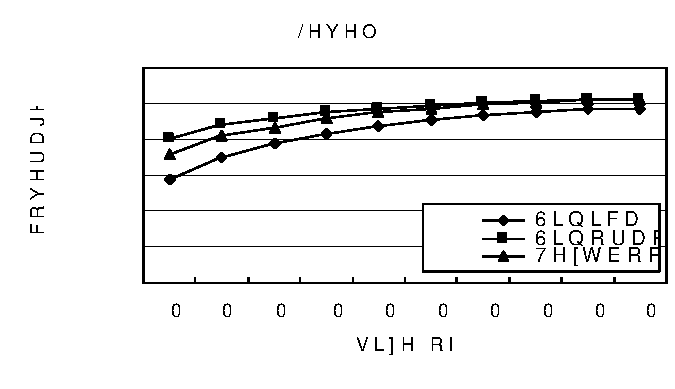
\includegraphics[width=\textwidth]{img/图1.pdf}
        \caption{WA coverage rate of Level-6.}
        \label{fig:figure1}
    \end{minipage}
    \hfill
    % 第二张图
    \begin{minipage}{0.45\textwidth}
        \centering
        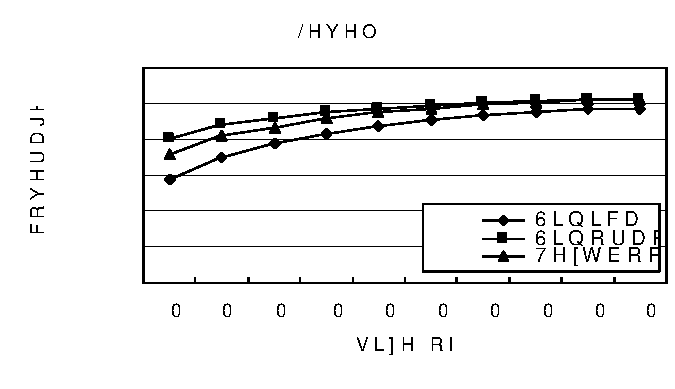
\includegraphics[width=\textwidth]{img/图2.pdf}
        \caption{Another figure.}
        \label{fig:figure2}
    \end{minipage}
\end{figure}

观察图3,投资与利率存在明显的负向关系,当利率升高时,投资降低;利率降低时,投资增加。消费与利率之间的关系不明显。图4显示,利率与实际有效汇率REER的关系方向不明朗实际有效汇率于 2005年开始有显著升值趋势,但这一区间的利率并未表现出持续上涨,可见,我国的人民币升值的主要原因并非来自利率。同时,人民币升值并没有造成净出口的减少,我国一直是一个贸易顺差的国家,理论上一国货币升值造成出口商品价格相对提高,进口商品价格相对下降,贸易将由顺差转向逆差(或者减少顺差,或者加大逆差),但在我国并没有出现这种情况,说明除了汇率之外,还有其他重要因素影响着我国的贸易水平,如较低的人工成本、规模效应等等。

\begin{figure}[h]
    \centering
    \begin{minipage}{0.45\textwidth}
        \centering
        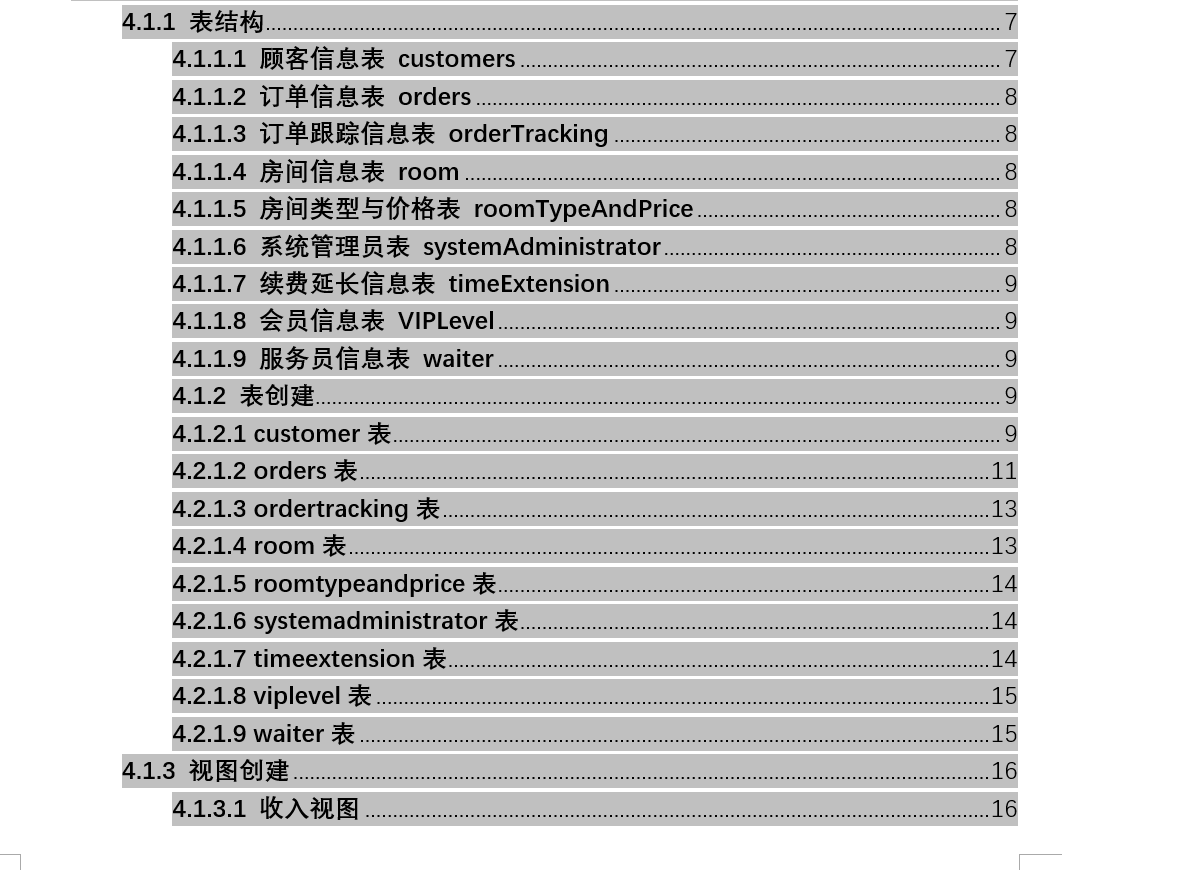
\includegraphics[width=\textwidth]{img/图3.png}
        \caption{WA coverage rate of Level-6.}
        \label{fig:figure3}
    \end{minipage}
    \hfill
    \begin{minipage}{0.45\textwidth}
        \centering
        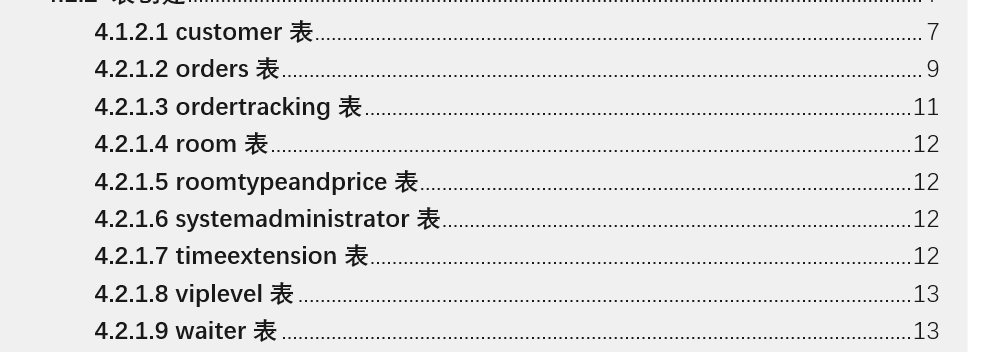
\includegraphics[width=\textwidth]{img/图4.png}
        \caption{Another figure.}
        \label{fig:figure4}
    \end{minipage}
\end{figure}
\textbf{}
\\
\\
\\
观察图5,我国的股票市场波动性较强,与M2增长率及利率不存在明显的相关关系。我们初步认为,股票市场价格与货币政策不相关。

观察图6,发现我国的房地产市场价格与利率呈现显著的负相关
\begin{figure}[h]
    \centering
    \begin{minipage}{0.45\textwidth}
        \centering
        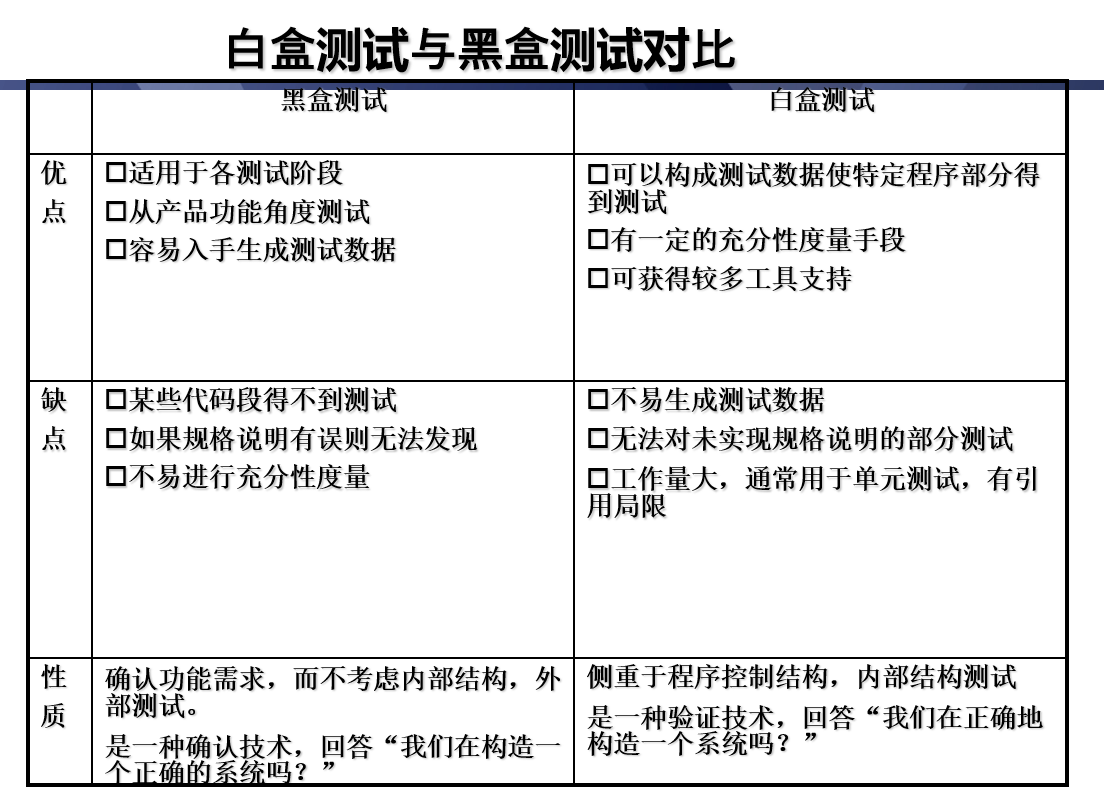
\includegraphics[width=\textwidth]{img/图5.png}
        \caption{WA coverage rate of Level-6.}
        \label{fig:figure3}
    \end{minipage}
    \hfill
    \begin{minipage}{0.45\textwidth}
        \centering
        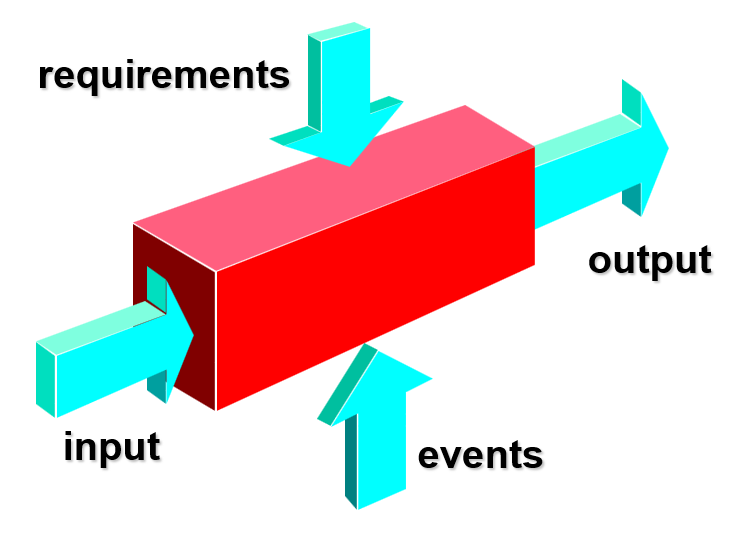
\includegraphics[width=\textwidth]{img/图6.png}
        \caption{Another figure.}
        \label{fig:figure4}
    \end{minipage}
\end{figure}

(2)设定符号约束

在本文的模型识别中,我们引入紧缩性货币政策冲击,研究紧缩性货币政策对宏观经济主要变量的影响。我们根据经济常识和公认的经济理论对冲击的影响效果进行约束。简单来看,货币当局实施紧缩性货币政策时,主要是通过提高市场利率,或者减少货币供应量(或降低货币供应量增长率);由于市场整体货币量减少,将进一步降低通货膨胀率,CPI下降;企业因需要承担更高的融资成本,因此投资(或其增长率)减少(或者降低);对于个人而言,利率的提升将提高储蓄倾向,而降低消费水平:对于整体产出而言,伴随投资和消费水平的降低,产出水平呈现下滑趋势。详见表1。

% Table Example
\begin{table}[h]
    \centering
    \begin{tabular}{lllrrr}
        \toprule
        \ \ 货币政策冲击\\
        \midrule
        Rate & + \\
        M2 & - \\
        GDP & - \\
        CPI & - \\
        Consumption & - \\
        Investment & - \\
        \bottomrule
    \end{tabular}
    \caption{符号约束}
\end{table}
\textbf{}\\\\\\\\\\\\
(3)实证估计

参考前文中介绍的 SVAR 模型(2)式,本文为了区分价格型货币政策及数量型货币政策,分别设置基础模型一和模型二:

模型一:$Y_1=(Rate, GDP,CPI,CON,Invest,HP,SP,NE, Reer)^'$

模型二: $Y_2=(GDP, CPI, CON, Invest,M2,HP,SP,NE, Reer)^'$

模型一中的变量分别代表: 利率、产出、价格、消费、投资、房价、股价、净出口和汇率,模型二中的 M2代表货币供应量,其他与模型一相同。本文利用 WinRATS8.0 软件进行该部分的实证检验。首先,在估计简化 VAR 模型时,我们利用 @VARLagSelect()函数及 AIC 准则选择模型的最优滞后阶数为1。且包含常数项,拟定抽样次数设置为20000,据上文中约定的识别条件对紧缩性货币政策的冲击进行识别,最终保留1000个符合约束的结构矩阵A.Scholl and Ulig(2008)认为符号约束识别冲击时,过长或过短的脉冲响应期限都不合适,以往文献均将脉冲响应期限设定在 20~35 之间,本文拟将脉冲响应期限设定为 nstep=25。模型变量 nvar=10,对于符合约束的期限,因为是季度变量,我们参考前人研究将约束期数设置为4,即 KMIN=1,KMAZ=4。

首先观察模型一得到的宏观经济变量对利率冲击的脉冲响应图(图7),我们可以得到如下结果: 提高利率对产出、通胀、消费和投资的即期效应均为负,这一点符合经济常识,紧缩性的货币政策会减少投资和消费,进一步降低产出,通胀率也随之下降,同时利率对这四种宏观经济变量的长期影响趋向于零。利率冲击对股价基本无影响,股市资产价格传导机制不可行,货币政策不能有效影响股市价格,进而不能通过托宾q效应(企业投资效应)、资产负债表效应或者是财富效应影响投资和消费,不能达到产出的预期效果,利率冲击虽然对汇率的即期影响为正,但对进出口基本无影响,说明通过汇率传导渠道影响进出口进而影响产出的渠道不畅通,提高利率的紧缩性货币政策,能够对房价产生短期影响,但很快房价有所反弹,说明利率对房价的调节作用不强。

再次观察模型二得到的宏观经济变量对货币供应量冲击的脉冲响应图(图8),我们发现:减少货币供应量对产出、通胀、消费和投资的即期效应均为负,这一点同样符合经济常识。长期来看,货币供应量(增长率)的降低能够对消费、投资和产出产生较长时间的影响。货币供应量同样对净出口和股价基本无影响,对房价影响与利率相似,短期影响为负,但会有价格反弹

(4)比较模型

方面增加社会融资规模季度增长率作为银行信贷的代理变量,城镇登记失业率作为失业率代理变量,考察货币政策冲击对银行信贷以及失业率的影响,而这两种指标公布时间较晚,因此比较模型的期限只能选用 2003Q1-2019Q4的数据;另外一方面,删除股票市场价格变量和净出口变量;最后,我们通过期限调整比较上述变量对货币政策冲击的反应,观察近年来货币政策效果是否发生变化,发生了哪些变化。

\begin{figure}[h]
    \centering
    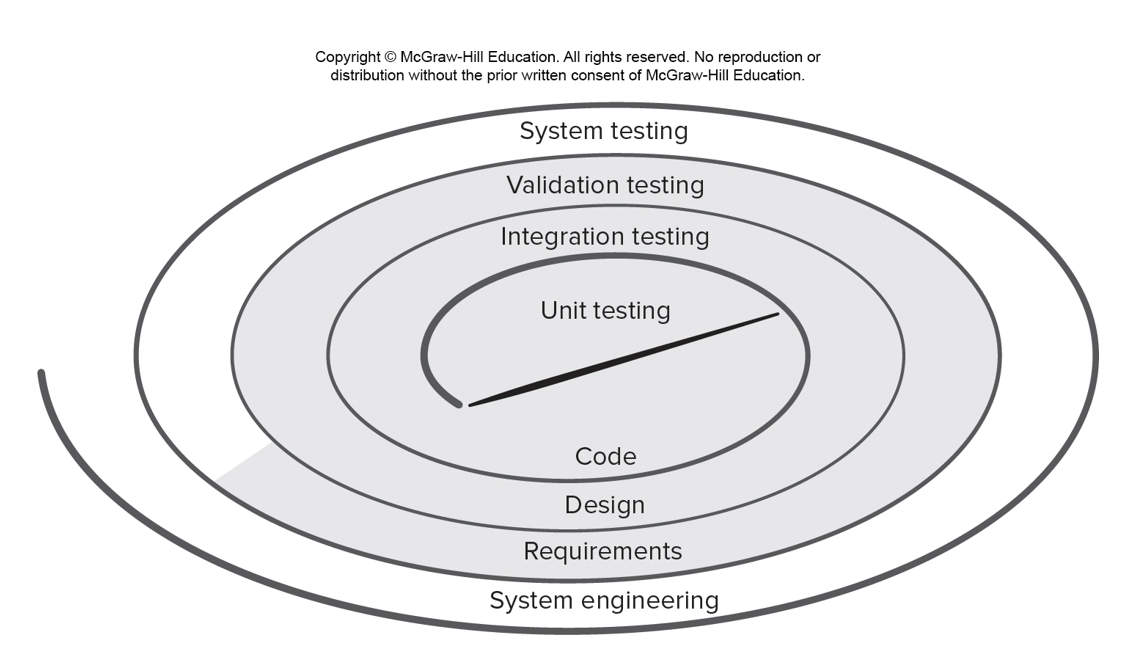
\includegraphics[width=0.8\textwidth]{img/图7.png}
    \caption{WA coverage rate of Level-6.}
\end{figure}
\begin{figure}[h]
    \centering
    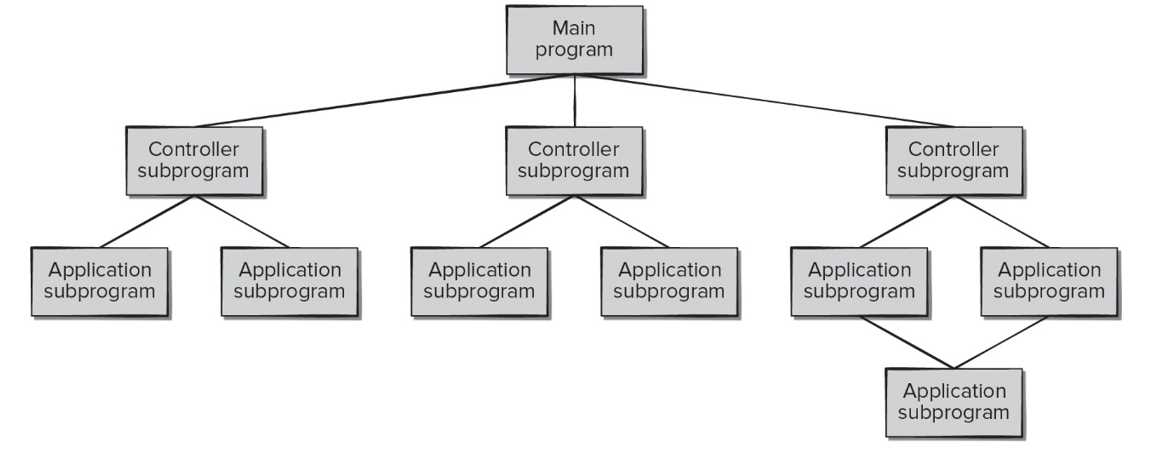
\includegraphics[width=0.8\textwidth]{img/图8.png}
    \caption{WA coverage rate of Level-6.}
\end{figure}
\textbf{}\\



建立比较模型三和模型四:

模型三:$Y_3=(Rate,GDP,CPI, CON,Invest,HP, Reer, Credit, Unemployment)^'$

\\
模型四:$Y_4=(GDP, CPI, CON,Invest, M2,HP,Reer, Credit, Unemployment)^'$

\\
模型三脉冲响应期限依然选定为 nstep=25,模型四脉冲响应期限依然选定为nstep=40(为了能够更好观察收敛性),模型变量 nvar-9,KMIN=1,KMAZ=4。

通过观察和对图9与图7比较发现:第一,利率对投资的即期影响下降,1996Q1-2019Q4(时段 1)的即期影响约3个单位,2003Q1-2019Q4(时段 2)的即期影响不到 2.5 个单位;第二,利率冲击对社会融资规模只有短期影响,但是很快在第一期和第二期影响消失。一般来讲,利率提高社会融资成本提高,融资规模应降低,但鉴于我国除了银行外,还存在大规模的影子银行,而影子银行的成本受市场基准利率的影响较小,我们采用的社会融资总规模数据包含了影子银行融资因此导致了此图中影响很快趋于零的结论:第三,利率冲击对失业率的影响为负,一单位的利率冲击对失业率产生约-0.01单位的影响,且这种影响会有持续性。第四,利率冲击对房价的影响在时段2有所加强。

通过观察和对图10与图8比较发现:第一,货币供应量对产出、投资、消费的即期影响变小说明近些年来货币供应量的政策效果有所下降。第二,货币供应量冲击对社会融资规模同样是短期负向影响,但很快影响趋于零。一般来讲,货币供应量的降低能够减少市场流动性,导致融资利率提高,社会融资规模对应下降,目前的冲击结果同样说明有其他因素阻碍了这种传导,作者认为与近年来发展的影子银行业务相关。第三,货币供应量冲击对失业率的长期影响为负,一单位的货币供应量冲击对失业率产生约-0.02单位的影响,第四,房价对货币供应量冲击的反应即期不明显,长期显著为负,货币供应量对汇率短期影响为正,但很快影响变小并趋于零。

\begin{figure}[h]
    \centering
    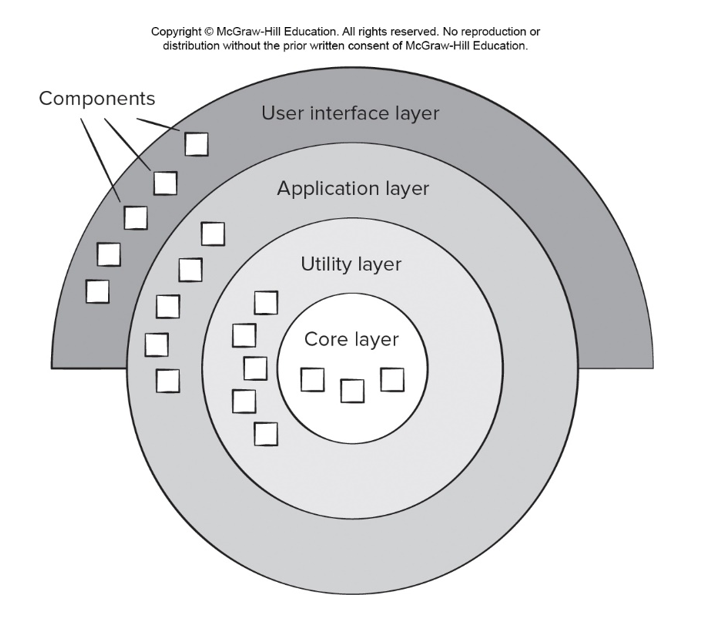
\includegraphics[width=0.8\textwidth]{img/图9.png}
    \caption{WA coverage rate of Level-6.}
\end{figure}
\begin{figure}[h]
    \centering
    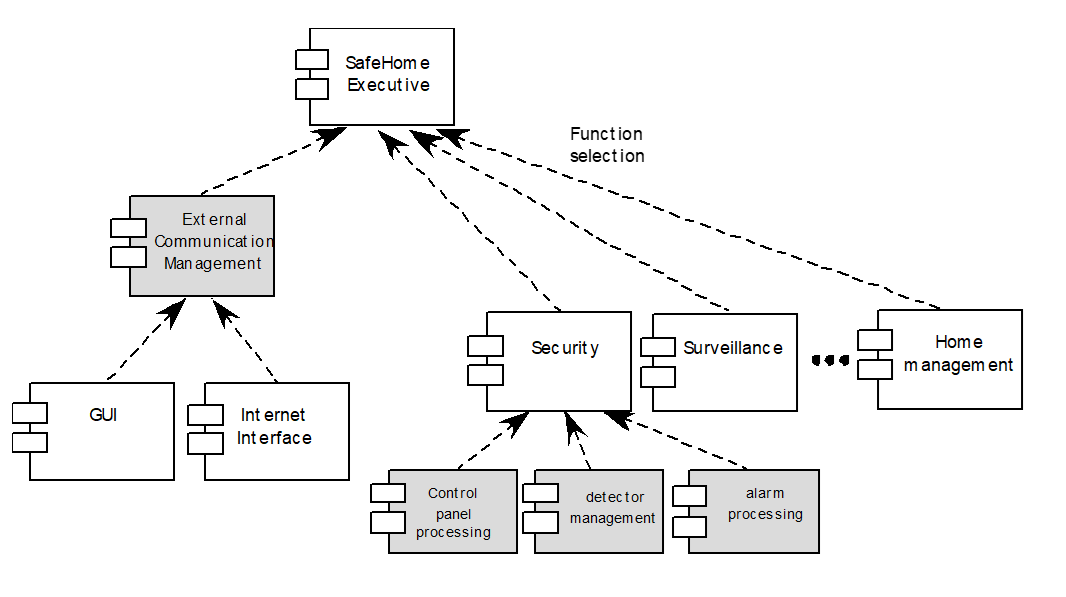
\includegraphics[width=0.8\textwidth]{img/图10.png}
    \caption{WA coverage rate of Level-6.}
\end{figure}

(5)稳健性检验
为检验模型的稳健性,本文从变量替换和约束期限调整两方面进行检验:首先,将七天同业拆借利率替换为一年期存款利率,重新对模型一进行识别,得到的结果与原模型结果基本一致;其次,作者将符号约束的期限调整为2期,即KMAX=2,对冲击发生后的半年的反应符号进行约束,得到的结果未发生实质变化。因此,作者认为以上模型是稳健的。

\section{不同货币政策的时变冲击效应}
This research was supported in part by National Science Council under Grant NSC 95-2422-H-001-008- and National Digital Archives Program Grant 95-0210-29-戊-13-09-00-2.

% References
\bibliography{references}
\begin{figure}[h]
    \centering
    \includegraphics[width=0.8\textwidth]{figure1.pdf}
    \caption{WA coverage rate of Level-6.}
\end{figure}
\end{document}
